\begin{figure}[!h]
    \centering
    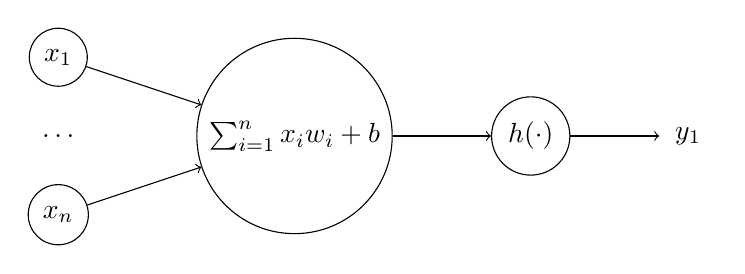
\begin{tikzpicture}
        \node[draw, circle] (x1) {$x_1$};
        \node[draw=none, circle, below of=x1] (dots) {$\dots$};
        \node[draw, circle, below of=dots] (xn) {$x_n$};
        \node[draw, circle, right of=dots, xshift=2cm] (sum) {$\sum_{i=1}^n x_iw_i + b$};
        \node[draw, circle, right of=sum, xshift=2cm] (activ) {$h(\cdot)$};
        \node[draw=none, circle, right of=activ, xshift=1cm] (out) {$y_1$};
        \draw[->] (x1) -- (sum);
        \draw[->] (xn) -- (sum);
        \draw[->] (sum) -- (activ);
        \draw[->] (activ) -- (out);
    \end{tikzpicture}
    \caption{Information flow through one hidden neuron in an MLP. $h(\cdot)$ represents an activation function.}
    \label{fig:mlp}
\end{figure}